\documentclass[aspectratio=169,10pt]{beamer}

\usetheme{Madrid}
\usecolortheme{beaver}
\useinnertheme{rectangles}

\usepackage{booktabs}
\usepackage{amsmath,amssymb}
\usepackage{tikz}
\usepackage{pgfplots}

\pgfplotsset{compat=1.18}
\usetikzlibrary{arrows.meta,positioning,fit,backgrounds,calc}

\setbeamertemplate{navigation symbols}{}
\setbeamertemplate{bibliography item}[text]
\setbeamerfont{footnote}{size=\scriptsize}
\setbeamercovered{transparent=25}

\newcommand{\sysname}{Tideline}

\title[\sysname]{\sysname: Ephemeris-Guided Congestion Control for\\ Low Earth Orbit Links}
\subtitle{Turning a predictable outage into a scheduling input}
\author[Vieira-Tan et al.]{Marisol Vieira-Tan \and Kwabena Osei-Brempong \and Helle Sandvik}
\institute[Ardmore IT]{Networked Systems Laboratory\\ Ardmore Institute of Technology}
\date{Workshop on Space Networking, March 2026}

\begin{document}

\begin{frame}[plain]
  \titlepage
\end{frame}

\begin{frame}{Outline}
  \tableofcontents
\end{frame}

\section{Why LEO breaks congestion control}

\begin{frame}{A low orbit link is not a lossy link}
  \begin{itemize}
    \item<1-> A terminal in a dense low orbit constellation changes serving satellite every 12 to 18 seconds.
    \item<2-> Each change moves the round trip time by 15 to 40 ms and the available capacity by up to 60 percent.
    \item<3-> Nothing about that is congestion. The path simply became a different path.
    \item<4-> Every deployed controller we tested reads it as congestion anyway, and backs off.
  \end{itemize}
  \vspace{0.5em}
  \onslide<4->{
    \begin{block}{Claim}
      The handover schedule is public, periodic, and known several minutes in advance.
      A controller that ignores it is discarding the single most useful signal on the path.
    \end{block}
  }
\end{frame}

\begin{frame}{What a handover looks like to the sender}
  \centering
  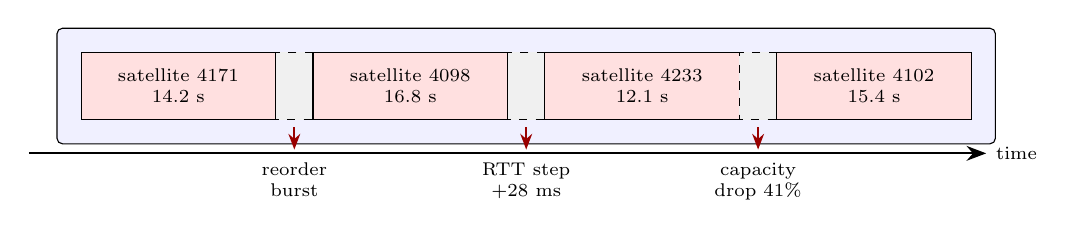
\begin{tikzpicture}[
      scale=0.95, transform shape,
      pass/.style={draw,fill=red!12,minimum height=9mm,minimum width=26mm,align=center,font=\scriptsize},
      gap/.style={draw,dashed,fill=gray!12,minimum height=9mm,minimum width=5mm},
      ev/.style={-{Stealth[length=2mm]},thick,red!60!black},
    ]
    \draw[-{Stealth[length=2.5mm]},thick] (-0.4,0) -- (12.4,0) node[right,font=\scriptsize] {time};
    \node[pass] (a) at (1.6,0.9) {satellite 4171\\\scriptsize 14.2 s};
    \node[gap]  (g1) at (3.15,0.9) {};
    \node[pass] (b) at (4.7,0.9) {satellite 4098\\\scriptsize 16.8 s};
    \node[gap]  (g2) at (6.25,0.9) {};
    \node[pass] (c) at (7.8,0.9) {satellite 4233\\\scriptsize 12.1 s};
    \node[gap]  (g3) at (9.35,0.9) {};
    \node[pass] (d) at (10.9,0.9) {satellite 4102\\\scriptsize 15.4 s};

    \foreach \x in {3.15,6.25,9.35} {
      \draw[ev] (\x,0.35) -- (\x,0.05);
    }
    \node[font=\scriptsize,anchor=north,align=center] at (3.15,0.0) {reorder\\burst};
    \node[font=\scriptsize,anchor=north,align=center] at (6.25,0.0) {RTT step\\$+28$ ms};
    \node[font=\scriptsize,anchor=north,align=center] at (9.35,0.0) {capacity\\drop 41\%};

    \begin{scope}[on background layer]
      \node[draw,rounded corners=2pt,fill=blue!6,fit=(a)(d),inner sep=3mm] {};
    \end{scope}
  \end{tikzpicture}

  \vspace{0.8em}
  \begin{itemize}
    \item<2-> The gaps are 80 to 220 ms of near total loss, not a queue filling up.
    \item<3-> A loss based controller halves its window. A delay based controller reads the RTT step as a growing queue and halves it too.
  \end{itemize}
\end{frame}

\begin{frame}{Measured cost of the misreading}
  \centering
  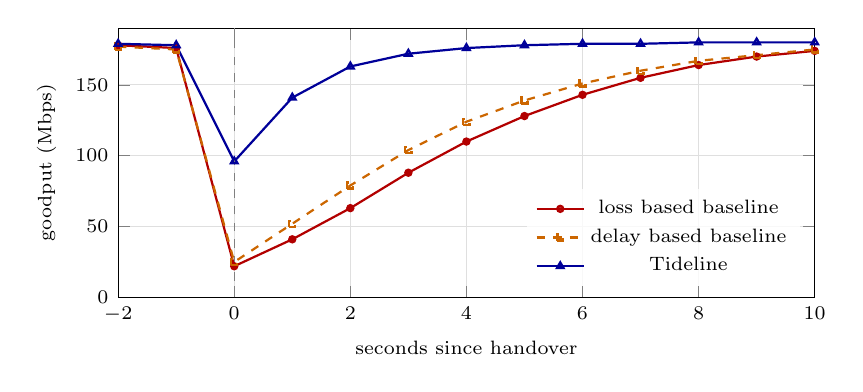
\begin{tikzpicture}
    \begin{axis}[
        width=0.86\linewidth, height=5.0cm,
        xlabel={seconds since handover},
        ylabel={goodput (Mbps)},
        xmin=-2, xmax=10, ymin=0, ymax=190,
        grid=both, grid style={gray!25},
        legend style={font=\scriptsize,at={(0.98,0.04)},anchor=south east,draw=none,fill=white,fill opacity=0.8,text opacity=1},
        tick label style={font=\scriptsize},
        label style={font=\scriptsize},
      ]
      \addplot[thick,mark=*,mark size=1.1pt,red!70!black] coordinates {
        (-2,178) (-1,176) (0,22) (1,41) (2,63) (3,88) (4,110) (5,128) (6,143) (7,155) (8,164) (9,170) (10,174)
      };
      \addlegendentry{loss based baseline}
      \addplot[thick,dashed,mark=square,mark size=1.1pt,orange!80!black] coordinates {
        (-2,177) (-1,175) (0,25) (1,52) (2,79) (3,104) (4,124) (5,139) (6,151) (7,160) (8,167) (9,171) (10,175)
      };
      \addlegendentry{delay based baseline}
      \addplot[thick,mark=triangle,mark size=1.4pt,blue!60!black] coordinates {
        (-2,179) (-1,178) (0,96) (1,141) (2,163) (3,172) (4,176) (5,178) (6,179) (7,179) (8,180) (9,180) (10,180)
      };
      \addlegendentry{\sysname}
      \draw[gray,dashed] (axis cs:0,0) -- (axis cs:0,190);
    \end{axis}
  \end{tikzpicture}

  \vspace{0.4em}
  \footnotesize
  Mean over 1{,}840 handovers on the emulated constellation. Recovery to 95 percent of
  pre-handover goodput takes 8.4 s for the loss based baseline and 1.6 s for \sysname.
\end{frame}

\section{Design}

\begin{frame}{\sysname{} in one picture}
  \centering
  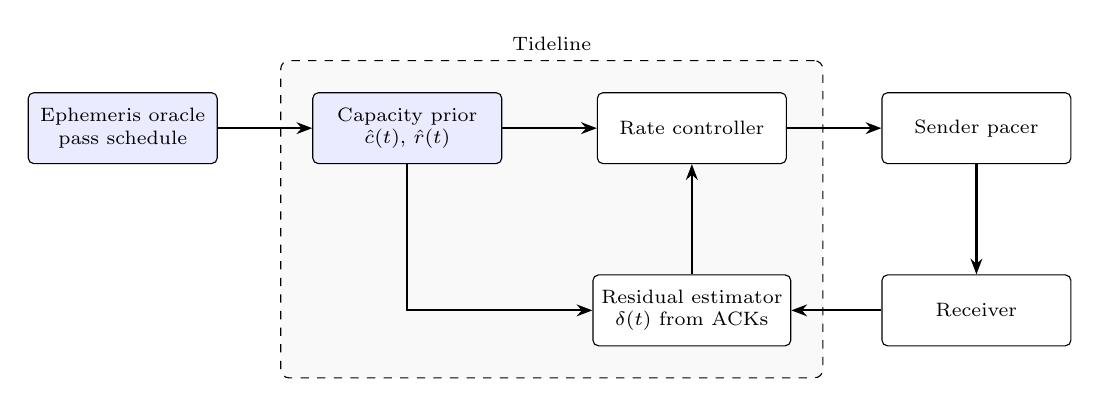
\begin{tikzpicture}[
      node distance=7mm and 12mm,
      box/.style={draw,rounded corners=2pt,align=center,font=\scriptsize,
                  minimum height=9mm,minimum width=24mm,inner xsep=3pt,fill=white},
      flow/.style={-{Stealth[length=2mm]},thick},
    ]
    \node[box,fill=blue!8] (eph) {Ephemeris oracle\\\scriptsize pass schedule};
    \node[box,right=of eph,fill=blue!8] (prior) {Capacity prior\\\scriptsize $\hat{c}(t)$, $\hat{r}(t)$};
    \node[box,right=of prior] (ctrl) {Rate controller};
    \node[box,right=of ctrl] (send) {Sender pacer};
    \node[box,below=14mm of ctrl] (res) {Residual estimator\\\scriptsize $\delta(t)$ from ACKs};
    \node[box,below=14mm of send] (recv) {Receiver};

    \draw[flow] (eph) -- (prior);
    \draw[flow] (prior) -- (ctrl);
    \draw[flow] (ctrl) -- (send);
    \draw[flow] (send) -- (recv);
    \draw[flow] (recv) -- (res);
    \draw[flow] (res) -- (ctrl);
    \draw[flow] (prior.south) |- ($(res.west)+(-0.6,0)$) -- (res.west);

    \begin{scope}[on background layer]
      \node[draw,dashed,rounded corners=3pt,fill=gray!5,fit=(prior)(ctrl)(res),
            inner sep=4mm,label={[font=\scriptsize]above:\sysname}] {};
    \end{scope}
  \end{tikzpicture}

  \vspace{0.6em}
  \begin{itemize}
    \item<2-> The prior is open loop and cheap. It never sees an ACK.
    \item<3-> The residual is closed loop and corrects the prior where the geometry is wrong.
    \item<4-> Neither component can starve the other: the controller clamps the prior to the residual's confidence interval.
  \end{itemize}
\end{frame}

\begin{frame}{The capacity prior}
  Given the serving satellite's elevation angle $\theta(t)$ and slant range $d(t)$ from the
  published ephemeris, the prior predicts a link rate
  \begin{equation}
    \label{eq:prior}
    \hat{c}(t) = c_{0}\,\frac{\sin \theta(t)}{\sin \theta_{0}}
                 \left(\frac{d_{0}}{d(t)}\right)^{2}
                 \bigl(1 - \mathbb{1}[t \in H]\bigr),
  \end{equation}
  where $H$ is the union of handover windows and $c_0, d_0, \theta_0$ are calibrated once per terminal.

  \pause
  \vspace{0.6em}
  Two properties matter more than the fit quality:
  \begin{enumerate}
    \item<2-> $\hat{c}$ is a \emph{schedule}, so the pacer can drain its queue \emph{before} the gap
      rather than discovering it afterwards.
    \item<3-> $\hat{c}$ is wrong in a bounded way. Rain fade and terminal obstruction only ever
      reduce the true rate, never raise it, so the prior is an upper bound.
  \end{enumerate}
  \onslide<4->{
    \begin{block}{Consequence}
      The controller may treat $\hat{c}$ as a ceiling and use the residual purely to move downward,
      which removes the usual risk of an over-confident model driving the sender into loss.
    \end{block}
  }
\end{frame}

\begin{frame}{The residual estimator}
  \begin{columns}[T]
    \begin{column}{0.55\textwidth}
      \begin{itemize}
        \item<1-> Over a 400 ms window the estimator fits
          $\delta = \log\bigl(c_{\text{obs}} / \hat{c}\bigr)$ with a Kalman filter whose
          process noise is keyed to the time until the next scheduled handover.
        \item<2-> Far from a handover, the filter trusts observations.
        \item<3-> Within 1 s of a scheduled handover, process noise is raised by $12\times$ so a
          transient is not absorbed into the steady state estimate.
        \item<4-> Sending rate is $r(t) = \hat{c}(t)\exp(\delta(t)) \cdot \gamma$ with headroom
          $\gamma = 0.92$.
      \end{itemize}
    \end{column}
    \begin{column}{0.45\textwidth}
      \centering
      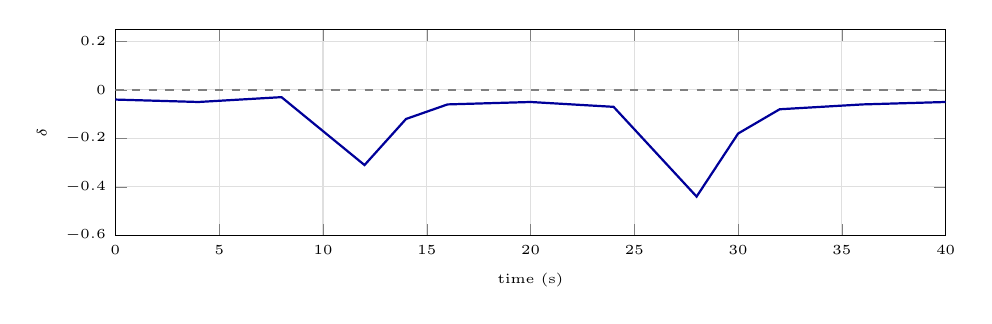
\begin{tikzpicture}
        \begin{axis}[
            width=\linewidth, height=4.2cm,
            xlabel={time (s)}, ylabel={$\delta$},
            xmin=0, xmax=40, ymin=-0.6, ymax=0.25,
            grid=both, grid style={gray!25},
            tick label style={font=\tiny},
            label style={font=\tiny},
          ]
          \addplot[thick,blue!60!black] coordinates {
            (0,-0.04) (4,-0.05) (8,-0.03) (12,-0.31) (14,-0.12) (16,-0.06)
            (20,-0.05) (24,-0.07) (28,-0.44) (30,-0.18) (32,-0.08) (36,-0.06) (40,-0.05)
          };
          \addplot[gray,dashed,thick] coordinates {(0,0) (40,0)};
        \end{axis}
      \end{tikzpicture}
      \scriptsize The two excursions are a rain cell at $t=12$ and a terminal obstruction at $t=28$,
      neither of which appears in the ephemeris.
    \end{column}
  \end{columns}
\end{frame}

\begin{frame}{Deployment shape}
  \begin{itemize}
    \item<1-> \sysname{} is 2{,}100 lines of userspace code and one kernel pacing hook. No change to the receiver.
    \item<2-> The ephemeris feed is a 40 kB two line element set refreshed every six hours, or 14 bytes
      per second of amortised traffic.
    \item<3-> If the feed is stale or absent, the prior degrades to a constant and \sysname{} falls back to
      a standard delay based loop. We measured that fallback path explicitly, see slide~\ref{fig:fallback}.
    \item<4-> Calibration of $c_0, d_0, \theta_0$ takes 90 seconds at terminal install time and is not
      repeated.
  \end{itemize}
\end{frame}

\section{Evaluation}

\begin{frame}{Setup}
  \begin{itemize}
    \item Emulated constellation of 1{,}584 satellites at 550 km, propagated from published orbital
      elements, driving a link emulator with per-pass capacity and delay traces.
    \item 40 terminals at latitudes from $12^{\circ}$ to $61^{\circ}$, twelve hours of wall clock time
      per configuration, three seeds.
    \item Baselines: a loss based controller in the style of CUBIC~\cite{ha2008cubic}, a model based
      controller in the style of BBR~\cite{cardwell2016bbr}, and a learned controller in the style of
      Vivace~\cite{dong2018vivace}.
    \item Workloads: bulk transfer, a 2 Mbps constant bitrate video flow, and a request and response
      trace with 8 kB objects.
  \end{itemize}
\end{frame}

\begin{frame}{Main result}
  \begin{table}
    \centering
    \small
    \begin{tabular}{lrrrr}
      \toprule
      Controller & Goodput (Mbps) & p99 RTT (ms) & Retransmit (\%) & Jain fairness \\
      \midrule
      Loss based       & 96.4  & 412 & 2.81 & 0.88 \\
      Model based      & 121.7 & 268 & 1.44 & 0.91 \\
      Learned          & 118.2 & 301 & 1.92 & 0.79 \\
      \sysname{} (prior only)  & 149.3 & 208 & 1.10 & 0.93 \\
      \sysname{}       & \textbf{166.9} & \textbf{147} & \textbf{0.62} & \textbf{0.94} \\
      \bottomrule
    \end{tabular}
  \end{table}

  \vspace{0.4em}
  \begin{itemize}
    \item<2-> Median goodput improves $1.73\times$ over the strongest baseline.
    \item<3-> The p99 RTT reduction of 45 percent is the number operators care about, and it comes
      almost entirely from draining before a scheduled gap.
    \item<4-> Fairness is measured against three competing \sysname{} flows on one terminal.
  \end{itemize}
\end{frame}

\begin{frame}{Where the gain comes from}
  \centering
  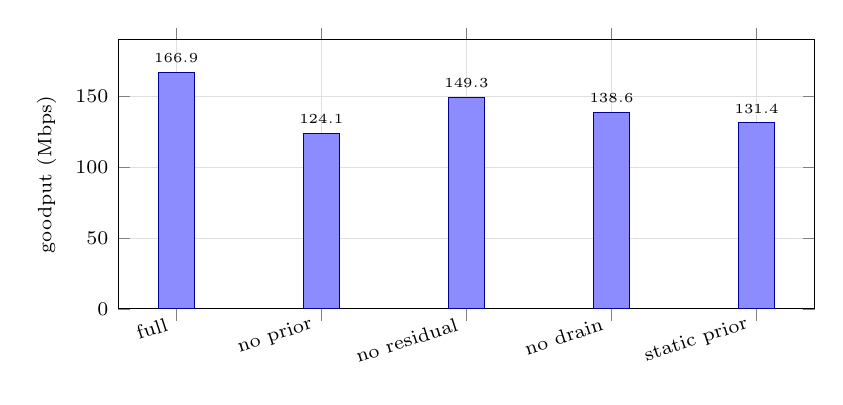
\begin{tikzpicture}
    \begin{axis}[
        ybar,
        width=0.86\linewidth, height=5.0cm,
        bar width=13pt,
        ylabel={goodput (Mbps)},
        symbolic x coords={full,no prior,no residual,no drain,static prior},
        xtick=data,
        ymin=0, ymax=190,
        nodes near coords, nodes near coords style={font=\tiny},
        grid=major, grid style={gray!25},
        tick label style={font=\scriptsize},
        label style={font=\scriptsize},
        x tick label style={rotate=18,anchor=east},
      ]
      \addplot[fill=blue!45,draw=blue!60!black] coordinates {
        (full,166.9) (no prior,124.1) (no residual,149.3) (no drain,138.6) (static prior,131.4)
      };
    \end{axis}
  \end{tikzpicture}

  \vspace{0.3em}
  \begin{itemize}
    \item<2-> Removing the prior costs the most, which is the point of the paper.
    \item<3-> Removing the pre-handover drain costs 17 percent of goodput and doubles p99 RTT.
  \end{itemize}
\end{frame}

\begin{frame}{Fairness against non-\sysname{} traffic}
  \begin{columns}[T]
    \begin{column}{0.5\textwidth}
      \begin{itemize}
        \item<1-> A scheduler that knows the future can starve one that does not.
        \item<2-> With headroom $\gamma = 0.92$ and the residual clamp, a competing model based flow
          keeps 0.87 of its solo share.
        \item<3-> Raising $\gamma$ to 1.0 raises \sysname{} goodput by 4 percent and drops the
          competing flow to 0.61 of solo share. We do not recommend it.
      \end{itemize}
    \end{column}
    \begin{column}{0.5\textwidth}
      \centering
      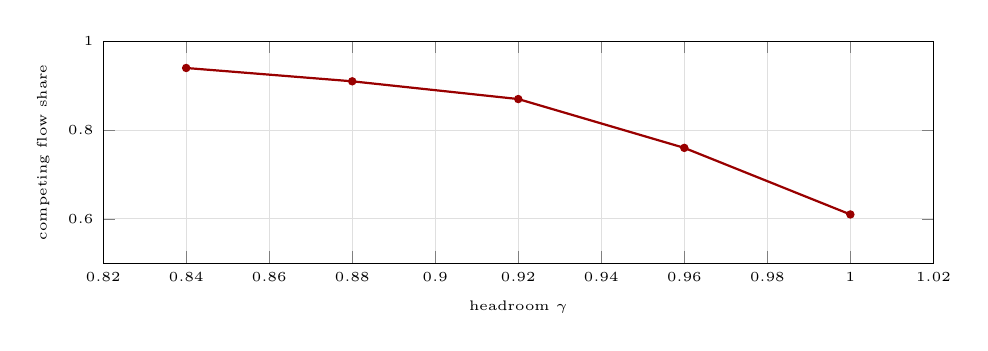
\begin{tikzpicture}
        \begin{axis}[
            width=\linewidth, height=4.4cm,
            xlabel={headroom $\gamma$}, ylabel={competing flow share},
            xmin=0.82, xmax=1.02, ymin=0.5, ymax=1.0,
            grid=both, grid style={gray!25},
            tick label style={font=\tiny}, label style={font=\tiny},
          ]
          \addplot[thick,mark=*,mark size=1.1pt,red!60!black] coordinates {
            (0.84,0.94) (0.88,0.91) (0.92,0.87) (0.96,0.76) (1.00,0.61)
          };
        \end{axis}
      \end{tikzpicture}
    \end{column}
  \end{columns}
\end{frame}

\section{Limitations}

\begin{frame}{What we could not fix}
  \begin{enumerate}
    \item<1-> \textbf{Sparse constellations.} Below roughly 400 satellites the pass gaps exceed one
      second and no amount of draining hides them. \sysname{} matches the baselines and does not beat them.
    \item<2-> \textbf{Ground segment congestion.} The prior models the space link only. When the gateway
      is the bottleneck the prior is a useless ceiling and all the work falls to the residual.
    \item<3-> \textbf{Adversarial scheduling.} An operator that reassigns terminals off the published
      schedule invalidates the prior within one window. The residual recovers in about 900 ms, which is
      worse than the baseline steady state.
  \end{enumerate}
  \onslide<3->{\vspace{0.4em}\footnotesize We report the third case because it decides whether \sysname{}
  should be enabled by default, and we think it should not be until the fallback margin narrows.}
\end{frame}

\begin{frame}{Conclusion}
  \begin{block}{The result}
    A handover is a scheduled event, not a congestion signal. Feeding the schedule into the rate
    controller as an upper bound recovers $1.73\times$ goodput and cuts tail latency by 45 percent
    without changing the receiver.
  \end{block}
  \pause
  \begin{block}{What we would do next}
    Extend the prior to the ground segment so that gateway capacity enters the same ceiling, and
    measure the fallback margin under deliberately unpublished reassignment.
  \end{block}
  \pause
  \begin{center}
    \large Questions.
  \end{center}
\end{frame}

\begin{frame}[allowframebreaks]{References}
  \footnotesize
  \bibliographystyle{plain}
  \bibliography{refs}
\end{frame}

\appendix

\begin{frame}{Backup: emulator fidelity}
  \begin{table}
    \centering
    \small
    \begin{tabular}{lrr}
      \toprule
      Quantity & Emulator & Terminal trace \\
      \midrule
      Median RTT (ms)            & 41.2  & 43.7 \\
      Handover interval (s)      & 14.9  & 15.4 \\
      Gap duration (ms)          & 118   & 131 \\
      Capacity step at gap (\%)  & 38.1  & 41.6 \\
      Loss outside gaps (\%)     & 0.09  & 0.14 \\
      \bottomrule
    \end{tabular}
  \end{table}
  \vspace{0.4em}
  \footnotesize
  The emulator is optimistic on gap duration by 13 ms and on loss by 0.05 percentage points, both
  of which favour the baselines rather than \sysname.
\end{frame}

\begin{frame}{Backup: behaviour with a stale ephemeris feed}
  \label{fig:fallback}
  \centering
  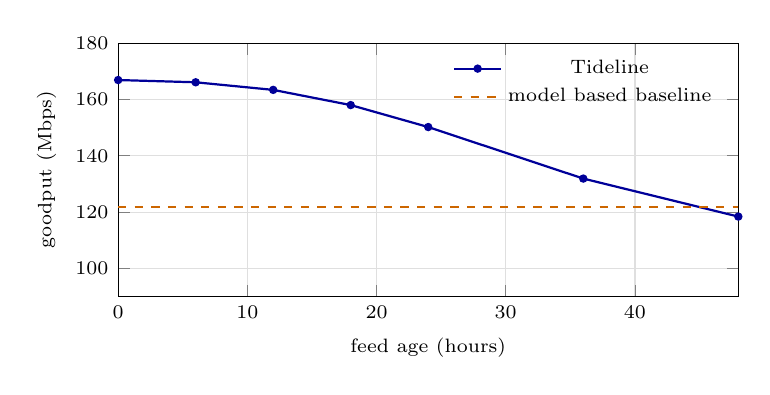
\begin{tikzpicture}
    \begin{axis}[
        width=0.78\linewidth, height=4.8cm,
        xlabel={feed age (hours)}, ylabel={goodput (Mbps)},
        xmin=0, xmax=48, ymin=90, ymax=180,
        grid=both, grid style={gray!25},
        legend style={font=\scriptsize,at={(0.98,0.98)},anchor=north east,draw=none,fill=none},
        tick label style={font=\scriptsize}, label style={font=\scriptsize},
      ]
      \addplot[thick,mark=*,mark size=1.1pt,blue!60!black] coordinates {
        (0,166.9) (6,166.1) (12,163.4) (18,158.0) (24,150.2) (36,131.9) (48,118.4)
      };
      \addlegendentry{\sysname}
      \addplot[thick,dashed,orange!80!black] coordinates {(0,121.7) (48,121.7)};
      \addlegendentry{model based baseline}
    \end{axis}
  \end{tikzpicture}

  \vspace{0.3em}
  \footnotesize
  \sysname{} stays ahead of the strongest baseline until the ephemeris is roughly 41 hours old.
  The refresh interval of six hours leaves a wide margin.
\end{frame}

\begin{frame}{Backup: parameters}
  \begin{table}
    \centering
    \small
    \begin{tabular}{llr}
      \toprule
      Symbol & Meaning & Value \\
      \midrule
      $\gamma$          & pacing headroom                & 0.92 \\
      $\theta_0$        & calibration elevation          & $40^{\circ}$ \\
      $d_0$             & calibration slant range        & 780 km \\
      $w$               & residual window                & 400 ms \\
      $\kappa$          & handover noise multiplier      & 12 \\
      $T_{\text{drain}}$ & pre-handover drain lead time  & 250 ms \\
      \bottomrule
    \end{tabular}
  \end{table}
  \vspace{0.4em}
  \footnotesize
  Every value was fixed on a held-out set of eight terminals and not tuned per experiment.
\end{frame}

\end{document}
